\documentclass[tikz,border=10pt]{standalone}
\usetikzlibrary{calc}
\begin{document}

\newcommand{\basejet}[1][]{

  \begin{scope}
    \draw (0,1) circle(0.3cm and 0.07cm);
  \end{scope}
  \draw[thick,gray,->,line cap =round] (0.0,0.02) -- node[left,font=\footnotesize] {} (90:1.4);
  \draw[gray,->,line cap =round] (0,0) -- node[left,font=\footnotesize] {} (80:1.3);
  \draw[gray,->,line cap =round] (0,0) -- node[left,font=\footnotesize] {} (100:1.3);

  \begin{scope}
    \clip (-1,0) rectangle (1,1);
    \draw (0,1) circle(0.3cm and 0.07cm);
  \end{scope}
  \draw[line cap =round] (0,0) -- (0.3,1);
  \draw[line cap =round] (0,0) -- (-0.3,1);
  #1
}

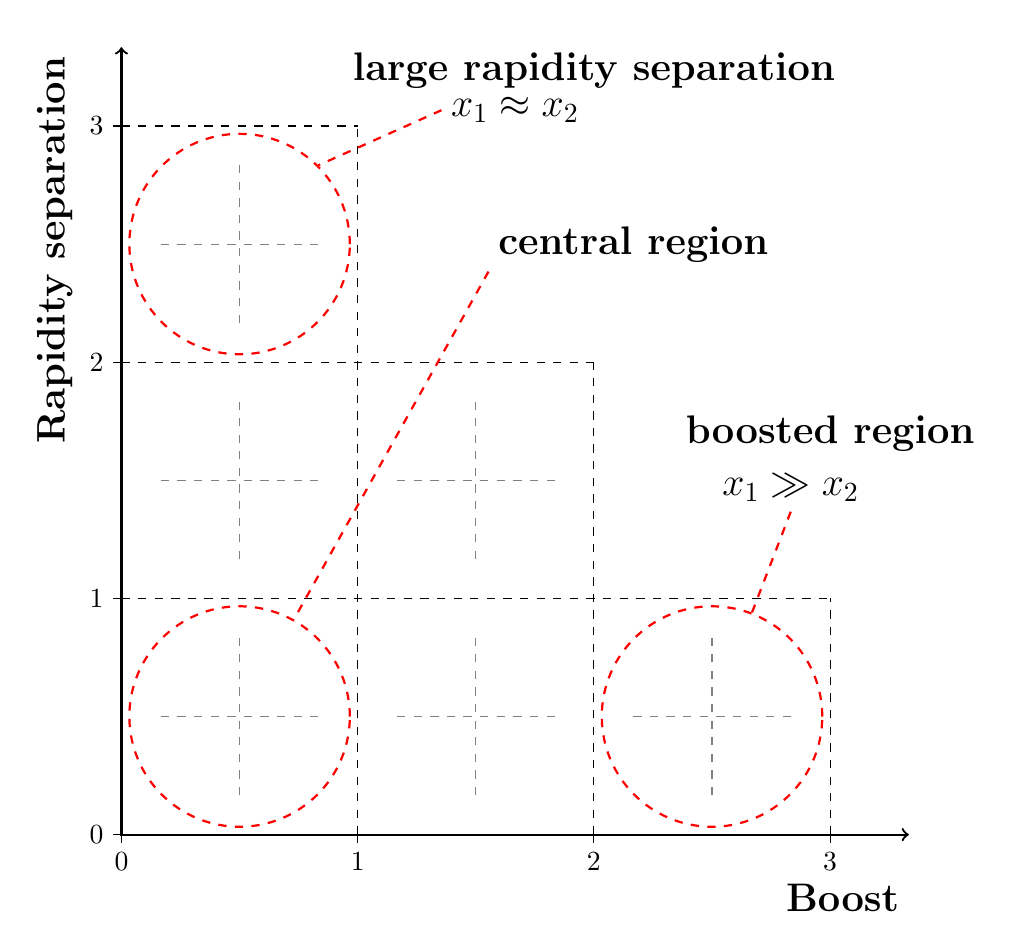
\begin{tikzpicture}
  \draw [<->,thick] (0,10) node (yaxis) [above right] {}
  |- (10,0) node (xaxis) [right] {};

  \node[anchor=south east,rotate=90] at (-0.5,10) {\Large \textbf{Rapidity separation}};
  \node[anchor=north east] at (10,-0.5) {\Large \textbf{Boost}};

  \draw (0,1pt) -- (0,-3pt) node[anchor=north] {0};
  \draw (3,1pt) -- (3,-3pt) node[anchor=north] {1};
  \draw (6,1pt) -- (6,-3pt) node[anchor=north] {2};
  \draw (9,1pt) -- (9,-3pt) node[anchor=north] {3};
  \draw (1pt,0) -- (-3pt,0) node[anchor=east] {0}; 
  \draw (1pt,3) -- (-3pt,3) node[anchor=east] {1}; 
  \draw (1pt,6) -- (-3pt,6) node[anchor=east] {2}; 
  \draw (1pt,9) -- (-3pt,9) node[anchor=east] {3}; 

  \draw[dashed] (3,0) -- (3,9);
  \draw[dashed] (6,0) -- (6,6);
  \draw[dashed] (9,0) -- (9,3);
  \draw[dashed] (0,3) -- (9,3);
  \draw[dashed] (0,6) -- (6,6);
  \draw[dashed] (0,9) -- (3,9);

  \begin{scope}[shift={(1.5,1.5)}]
    \draw[gray,dashed] (-1,0) -- node[left,font=\footnotesize] {} (1,0);
    \draw[gray,dashed] (0,-1) -- node[left,font=\footnotesize] {} (0,1);
    \basejet
    \begin{scope}[rotate=180]
      \basejet
    \end{scope}

  \end{scope}

  %yb1ys0


  \begin{scope}[shift={(4.5,1.5)}]
    \draw[gray,dashed] (-1,0) -- node[left,font=\footnotesize] {} (1,0);
    \draw[gray,dashed] (0,-1) -- node[left,font=\footnotesize] {} (0,1);
    \begin{scope}[rotate=-30]
      \basejet
    \end{scope}
    \begin{scope}[rotate=220]
      \basejet
    \end{scope}
  \end{scope}

  \begin{scope}[shift={(7.5,1.5)}]
    \draw[gray,dashed] (-1,0) -- node[left,font=\footnotesize] {} (1,0);
    \draw[gray,dashed] (0,-1) -- node[left,font=\footnotesize] {} (0,1);

    \begin{scope}[rotate=-60]
      \basejet
    \end{scope}
    \begin{scope}[rotate=240]
      \basejet
    \end{scope}
  \end{scope}

  \begin{scope}[shift={(1.5,4.5)}]
    \draw[gray,dashed] (-1,0) -- node[left,font=\footnotesize] {} (1,0);
    \draw[gray,dashed] (0,-1) -- node[left,font=\footnotesize] {} (0,1);

    \begin{scope}[rotate=30]
      \basejet
    \end{scope}
    \begin{scope}[rotate=210]
      \basejet
    \end{scope}
  \end{scope}

  \begin{scope}[shift={(4.5,4.5)}]
    \draw[gray,dashed] (-1,0) -- node[left,font=\footnotesize] {} (1,0);
    \draw[gray,dashed] (0,-1) -- node[left,font=\footnotesize] {} (0,1);

    \begin{scope}[rotate=0]
      \basejet
    \end{scope}
    \begin{scope}[rotate=240]
      \basejet
    \end{scope}
  \end{scope}

  \begin{scope}[shift={(1.5,7.5)}]
    \draw[gray,dashed] (-1,0) -- node[left,font=\footnotesize] {} (1,0);
    \draw[gray,dashed] (0,-1) -- node[left,font=\footnotesize] {} (0,1);

    \begin{scope}[rotate=60]
      \basejet
    \end{scope}
    \begin{scope}[rotate=240]
      \basejet
    \end{scope}
  \end{scope}

  \node[circle, draw, minimum size=2.8cm, thick, dashed, red] (hintA) at  (1.5,7.5) {};
  \node[] (hintAtext) at (5,9.2) {\Large $x_1 \approx x_2$};
  \node[] () at (6,9.7) {\Large \textbf{large rapidity separation}};
  \draw[thick, dashed, red] (hintAtext.west) -- (hintA.north east) ;

  \node[circle, draw, minimum size=2.8cm, thick, dashed, red] (hintA) at  (1.5,1.5) {};
  % \node[] () at (5,9.5) {\Large $x_1 \approx x_2$};
  \node[] (hintAtext) at (6.5,7.5) {\Large \textbf{central region}};
  \draw[thick, dashed, red] (hintAtext.south west) -- (hintA) ;

  \node[circle, draw, minimum size=2.8cm, thick, dashed, red] (hintA) at  (7.5,1.5) {};
  \node[] (hintAtext) at (8.5,4.4) {\Large $x_1 \gg x_2$};
  \node[] () at (9,5.1) {\Large \textbf{boosted region}};
  \draw[thick, dashed, red] (hintAtext.south) -- (hintA) ;



\end{tikzpicture}
\end{document}
